\documentclass[a4paper,11pt]{article}
\usepackage[utf8]{inputenc}
\usepackage[hungarian]{babel}
\usepackage{t1enc}
\usepackage[margin=2cm]{geometry}
\usepackage{graphicx}
\usepackage{amsmath}
\usepackage{amssymb}
\usepackage{mathtools}
\usepackage{setspace}
\usepackage{parskip}
\usepackage{tcolorbox}
\usepackage{mdframed}
\usepackage[hidelinks]{hyperref}
\usepackage{tikz}
\usetikzlibrary{automata, positioning}
\usepackage{enumerate}
\usepackage{ulem}
\usepackage{lipsum}
\usepackage{stuki}
\usepackage{stukicommands}
\usepackage{multirow}

%\onehalfspacing

\newtheorem{theorem}{tétel}[section]
\newtheorem{corollary}{következmény}
\newtheorem{proposition}{állítás}[section]
\newtheorem{definition}{definíció}[section]
\newtheorem{notation}{jelölés}[section]
\newtheorem{example}{példa}[section]
\newtheorem{remark}{megjegyzés}[section]

\newcommand{\setdivbar}{~ \middle\vert ~}
\newcommand{\emptyword}{\varepsilon}
\newcommand{\prodrule}[2]{#1 \longrightarrow #2}
\newcommand{\genword}[2]{\xRightarrow[{#1}]{#2}}
\newcommand{\partition}[1]{\stackrel{#1}{\sim}}

\DeclareMathOperator{\dotdot}{..}


\begin{document}

\author{\textsc{Nagy Sára} gyakorlatai alapján}
\title{\textbf{Formális nyelvek és a fordítóprogramok alapjai} \\ {\Large 2023/2024/2. félév, B szakirány} }
\date{\textit{Utolsó módosítás: \today}}

%\frontmatter
\maketitle

\section*{Előszó}

Ez a gyakorlati jegyzet a 2023/2024/2. félévben készült \textsc{Nagy Sára} tanárnő gyakorlatain, a B szakirányos \textit{Formális nyelvek és a fordítóprogramok alapjai} c. tantárgy keretein belül.

Bizonyos esetekben a feladatokat részletesebben vezettem le, adott esetben saját jelölésrendszert alkalmazva (amik nem szerepeltek a gyakorlatokon), hogy szemléletesebben be tudjam mutatni az egyes feladattípusokhoz tartozó algoritmusokat. Ha nem vagy benne biztos, hogy milyen részletességgel kér(het)ik számon ezeket a zárthelyiken, fordulj a gyakorlatvezetődhöz.

Igyekeztem a legjobb tudásom szerint összeállítani a jegyzetet, ennek ellenére előfordulhatnak benne elgépelések, hibák, stb. Ha találsz ilyet, kérlek értesíts e-mailben a(z) \href{mailto:ap3558@inf.elte.hu}{ap3558@inf.elte.hu} címen.

Sikeres felkészülést kívánok!

%\textit{\today}

\begin{flushright}
	\textit{Kiss-Bartha Nimród}
\end{flushright}

\tableofcontents

\newpage


\section{Formális nyelvek}

\subsection{Nyelv lezártjának meghatározása (nem hivatalos módszer)}

~\\[-2em]

\begin{mdframed}
	\textbf{Feladat}: Határozzuk meg egy nyelv lezártját.
	
	\textbf{Előfeltétel}: ($L$ véges nyelv legyen)
\end{mdframed}

Gyakorlatokon előforduló feladat, hogy határozzuk meg egy adott nyelv iteráltját. Általában nem egy olyan feladatról van szó, amit ránézésre könnyen megállapíthatunk, mindemellett koncentrációt igényel, emiatt könnyű elveszni a hasonló sztringek halmazában. Mindemellett a felsorolás is számít, ugyanis lexikografikusan várják el a zárthelyin. A programozó meg lusta, nem szeret sok időt tölteni ilyen feladatokkal. Erre javaslom a következő megoldást!

%~\\[-2.5em]

A szemléltetés kedvéért vegyük az alábbi nyelvet: $L := \{ \texttt{a}, \texttt{ab}, \texttt{cba} \}$.

	\begin{enumerate}
		\item lépés: $L^0 = L_\emptyword = \{ \emptyword \}$ és $L^1 = L$. Idáig elég egyszerű.
		\item lépés: határozzuk meg $L^2$-t. Ilyen kis nyelvnél még akár fejben is ki lehet találni, nagyobbaknál azonban gondban leszünk. Így ezen a kicsin mutatom be a módszert.
		
		Írjuk fel az $L$ szavait egy $(n+1) \times (n+1)$-es mátrixba ($n = |L|$), ahol a sorokba és oszlopokba helyezzük el a szavakat \textit{lexikografikusan}! Ezután a szavakat soronként és oszloponként konkatenálva töltsük ki a táblázatot!
		\begin{center}
			\begin{tabular}{|c|c|c|c|}
				\hline
				$LL$ & \texttt{a} & \texttt{ab}  & \texttt{cba}  \\
				\hline
				\texttt{a} & \texttt{aa} & \texttt{aab} & \texttt{acba}  \\
				\hline
				\texttt{ab} & \texttt{aba} & \texttt{abab} & \texttt{abcba}  \\
				\hline
				\texttt{cba} & \texttt{cbaa} & \texttt{cbaab} & \texttt{cbacba} \\
				\hline
			\end{tabular}
		\end{center}
		Innen kiolvashatjuk, hogy \[ L^2 = \{ \texttt{aa}, \texttt{aab}, \texttt{aba}, \texttt{abab}, \texttt{acba}, \texttt{cbaa}, \texttt{abcba}, \texttt{cbaab}, \texttt{cbacba} \}. \]
		\item lépés: elvégezzük a hatványraemelést a hatványozás definíciója szerint (azaz ha $n > 1$, akkor $L^n = L^{n-1}L$). Azt megállapítottuk, hogy nem számít, hogy balrekurzívan vagy jobbrekurzívan határozzuk meg a műveletet, mindkét módon helyes eredményeket kapunk. Ezt kihasználva úgy döntöttem, az $L^2$ elemeit a 1. sorban, az $L$ elemeit meg a 1. oszlopban sorakoztatom fel -- ami jobbrekurzív hatványozást jelent.
	\end{enumerate}
	\begin{center}
		\begin{small}
			\begin{tabular}{|c|c|c|c|c|c|c|c|c|c|}
				\hline
				$LL^2 $& \texttt{aa} & \texttt{aab} & \texttt{aba} & \texttt{abab} & \texttt{acba} & \texttt{cbaa} & \texttt{abcba} & \texttt{cbaab} & \texttt{cbacba} \\
				\hline
				\texttt{a} & $\texttt{a}^3$ & \texttt{aaab} & \texttt{aaba} & \texttt{aabab} & \texttt{aacba} & \texttt{acbaa} & \texttt{aabcba} & \texttt{acbaab} & \texttt{acbacba} \\
				\hline
				\texttt{ab} & \texttt{abaa} & \texttt{abaab} & \texttt{ababa} & $\texttt{ab}^3$ & \texttt{abacba} & \texttt{abcbaa} & \texttt{ababcba} & \texttt{abcbaab} & \texttt{abcbacba} \\
				\hline
				\texttt{cba} & \texttt{cbaaa} & \texttt{cbaaab} & \texttt{cbaaba} & \texttt{cbaabab} & \texttt{cbaacba} & \texttt{cbacbaa} & \texttt{cbaabcba} & \texttt{cbacbaab} & $\texttt{cba}^3$ \\
				\hline
			\end{tabular}
		\end{small}
	\end{center}
	
	A legnagyobb problémát ezúttal csak a lexikografikus felsorolás jelentheti, ugyanis eltérő hosszú szavak vannak az egyes $L^i$ halmazokban, mégha a legrövidebb hossz az halmazról halmazra nő. De még így is megfigyelhető egy olyan tendencia, hogy a táblázat bal felső sarkából elindulva egy olyan útvonalon járhatjuk be a cellákat, hogy azokból megkapjuk a szükséges sorrendet.
%\end{mdframed}

\newpage

\subsection{Nyelvtan típusának meghatározása}

Legyen $G := (N, T, P, S)$, ahol $T := \{ \texttt{a}, \texttt{b} \}$ és $P$ szabályai:
\begin{align*}
	&\prodrule{S}{\emptyword}, \\
	&\prodrule{S}{\texttt{a}S\texttt{b}}, \\
	&\prodrule{S}{SS}.
\end{align*}
Első lépésként azonosítsuk be az egyes szabályokról, hogy alakilak milyen típusú nyelvtanok szabályaihoz tartozhatnak! Ezeket felsorolhatjuk a szabályok mellé. 

Vegyük figyelembe, hogy egy szabály több nyelvtani típusnak is része lehet. Gondoljunk csak bele, a 0-ás típusú nyelvtant úgy definiáltuk, hogy nem vonatkozik rá semmilyen megkötés, így minden produkciós szabály automatikusan 0-ás típusú nyelvtannak része.
\begin{align*}
	&\prodrule{S}{\emptyword}& & \text{0, 1, \textbf{2}, 3} \\
	&\prodrule{S}{\texttt{a}S\texttt{b}}& & \text{0, \textbf{2}} \\
	&\prodrule{S}{SS}& & \text{0, \textbf{2}}
\end{align*}
Az első szabály mindegyik típusú nyelvtanban szerepelhet.

A második az 1-esben már nem szerepelhet, ugyanis megkötöttük, hogy az üres szót előállító szabályunk nem szerepelhet más szabály jobb oldalán. Márpedig az $S$ előállítha $\emptyword$-t és jobb oldalon szerepel. 3-as típusú azért nem lehet, mert az \fbox{\texttt{a}$S$\texttt{b}} jobb oldal nem illeszkedik bele egyik alakba sem:
\begin{itemize}
	\item az $S$ nemterminális után rögtön következik egy terminális szimbólum \\ (ezt az $\prodrule{A}{uB}$ $(A,B \in N, u \in T^*)$ forma nem engedi), 
	\item valamint a terminálisok közé közbeékelt $S$ nemterminális sem megengedett az $\prodrule{A}{u}$ $(u \in T^*)$ alaki megszorítás szerint.
\end{itemize}

Hasonló megfontolásokból következnek a 3. szabályra vonatkozó megállapítások.

Jelöljük ki azt a legmagasabb számot, amely az összes szabálynál szerepel. Ez fogja meghatározni, hogy milyen típusba esik bele a grammatikánk. Ebből megállapíthatjuk, hogy a $G$ egy 2-es típusú vagy környezetfüggetlen nyelvtan, azaz \[ G \in \mathcal{G}_2. ~~ \checkmark\]
Korábbról tudjuk, hogy \[ \mathcal{G}_3 \subseteq \mathcal{G}_2. \] Kérdés, hogy \textbf{tudunk-e 3-as típusú grammatikát adni ehhez a nyelvhez}. Ez azért egy fontos felvetés, ugyanis a célunk az, hogy \textit{a lehető legbelsőbb részhalmazba tudjunk ``átlépni''} (ez esetben a 3-as típusú grammatikák halmazába), ami a fordítóprogramok szempontjából egy óriási előnyt jelent.

Sajnos, meg kell előlegeznünk, hogy ehhez a nyelvhez \textit{nem tudunk $\mathcal{G}_3$-beli grammatikát adni}. Ezt csak később fogjuk tudni belátni.

A $G$ által generált nyelv 2-es típusú nyelv lesz, ezért \[L(G) \in \mathcal{L}_2\] teljesül. Ha netán mégis létezne hozzá $\mathcal{G}_3$-beli nyelvtan, akkor a \textbf{generált nyelv szigorú típusa} $L(G) \in \mathcal{L}_3$ lenne. De mivel nem tudunk ilyet adni, így a szigorú típusa $\mathcal{L}_2$.

\newpage

\subsection{Szó levezetése}

%\begin{mdframed}
	Legyen a levezetendő szó $u := \texttt{aabaabbb}$. Idézzük fel a $G$ nyelvtan produkciós szabályait:
	\begin{align*}
		&\prodrule{S}{\emptyword}, \\
		&\prodrule{S}{\texttt{a}S\texttt{b}}, \\
		&\prodrule{S}{SS}.
	\end{align*}
	Ha ezt a szót le tudjuk vezetni a $P$-beli szabályok véges szokszori alkalmazásával, akkor ez a szó eleme lesz a $G$ által generált nyelvnek.
	
	Ismerjük a nyelvtani szabályokat, ismerjük a startszimbólumot, valamint ismerjük a legyártandó szót is. Tehát valamilyen lépéssorozatból az alábbi összefüggést, levezetést kell megkapjuk:
	\[ S \genword{G}{*} \texttt{aabaabbb}. \]
	Egy kis ismétlés: a $\Longrightarrow$ alatt a $G$ azt jelenti, hogy a $G$ nyelvtan generálja a szót, ami egyértelmű kontextus esetén elhagyható. A $*$ meg azt, hogy véges sok lépésből vezethetjük le a szót.
	
	Induljunk ki az $S$-ből! Vizsgáljuk meg, melyik szabályokat tudjuk alkalmazni -- szakszóval ezt úgy mondjuk, hogy \textbf{mely szabályok \textit{tüzelőképesek}}. A mi esetünkben mindhárom tüzelőképes, így sok választási lehetőségünk van. Kezdetnek alkalmazzuk a 2. szabályt!
	\[ S \genword{G}{\text{2. szabály}} \texttt{a}S\texttt{b}. \]
	Ezután alkalmazzuk a 3. szabályt!
	\[ S \genword{G}{\text{2. szabály}} \texttt{a}S\texttt{b} \genword{G}{\text{3. szabály}} \texttt{a}SS\texttt{b}. \]
	Itt már két nemterminálisunk van, úgyhogy bármelyikkel folytathatjuk, nincs megszabva semmilyen sorrend. A lényeg, hogy létezzen egy véges lépéssorozata a szabályoknak, mellyel az $S$-ből a kívánt szóba el tudunk jutni -- és ez a szabálysorozat lehet tetszőlegesen egyszerű vagy feleslegesen hosszú, kacifántos és bonyolult. Ha van ilyen, akkor más létezik a szó a nyelvben.
	
	Itt az első $S$-re fogom alkalmazni a 2., majd az 1. szabályt.
	
	\[ S \genword{G}{\text{2.}} \texttt{a}S\texttt{b} \genword{G}{\text{3.}} \texttt{a}SS\texttt{b}. \genword{G}{\text{2. (első $S$-re)}} \texttt{aa}S\texttt{b}S\texttt{b} \genword{G}{\text{1. (első $S$-re)}} \texttt{aa}\emptyword\texttt{b}S\texttt{b} = \texttt{aa}\texttt{b}S\texttt{b}. \]
	
	Ismét egyetlen $S$ nemterminálisunk maradt. Ezekre a 2. szabályt fogom alkalmazni kétszer, majd végül az elsőt, hogy lezárjam a szót.
	
	\[ \texttt{aa}\texttt{b}S\texttt{b} \genword{G}{\text{2.}} \texttt{aaba}S\texttt{bb} \genword{G}{\text{2.}} \texttt{aabaa}S\texttt{bbb} \genword{G}{\text{1. (üres szavas szabály)}} \texttt{aabaa}\texttt{bbb}. ~~~ \checkmark \]
	
	Nem kell megijedni, ha más megoldást is találunk. Egy adott szót többféleképpen is levezethetünk. A $P$-beli produkciós szabályok valójában \textit{relációk}, nem függvények, ezért nondeterminisztikusak.
%\end{mdframed}

\textbf{\textit{Megjegyzés}}. Ha kicseréljük az \texttt{a}-t a \fbox{\texttt{(}} karakterre és a \texttt{b}-t a \fbox{\texttt{)}} karakterre, akkor megkapjuk pontosan a \textit{helyes zárójelezések nyelvé}t. Tehát, ha a levezetett szavunkban kicseréljük a szimbólumokat, akkor az alábbi eredményt kapjuk: \[ \Big( \big(\big) \big( () \big) \Big). \]

\newpage

\subsection{Epszilon-mentesítés ($\emptyword$-mentesítés)}

~\\[-2em]

\begin{mdframed}
	\textbf{Feladat}: Transzformáljuk át a $G \in \mathcal{G}_2$ (vagy $G \in \mathcal{G}_3$) nyelvtant úgy, hogy
	\begin{itemize}
		\item ha az $S$-ből közvetetten levezethető az $\emptyword$, akkor azt a $G$ egyetlen módon legyen képes előállítani,
		\item ha nem levezehthető az $S$-ből közvetetten az $\emptyword$, akkor szabaduljunk meg az $\emptyword$-szabályoktól.
	\end{itemize}
	
	\textbf{Előfeltétel}: A nyelvtan 2-es vagy 3-as típusú legyen.
\end{mdframed}

A feladathoz kapcsolódik egy tétel, így a megoldás maga ezen tétel bizonyításának az algoritmusa.

Szemléltessük az alábbi nyelvtanon!
\begin{flalign*}
	G : & ~~~~ \prodrule{S}{BA \mid \texttt{aa}} \\
		& ~~~~ \prodrule{A}{BB \mid \texttt{a}A\texttt{b}} \\
		& ~~~~ \prodrule{B}{\emptyword \mid S\texttt{b}A}
\end{flalign*}
Legyen $H_1$ halmaz, ami azon nemterminálisokat tartalmazza, melyekből közvetlenül levezethető az $\emptyword$ szó (más szóval, $\prodrule{A}{\emptyword}$ alakúakat tartalmaz).
\[ H_1 := \{ B \}, ~~~~~~~~~~ \text{ugyanis } \prodrule{B}{\emptyword}. \]
Ezt bővítjük iteratívan.
\begin{align*}
	H_2 & := H_1 \cup \{ A \} = \{ A, B \},  & \text{ugyanis $A$-ból $B$-be eljuthatunk.} \\
	H_3 & := H_2 \cup \{ S \} = \{ A, B, S \}, & \text{ugyanis $S$-ből $A$-ba (ahonnal $B$-be) eljuthatunk.}
\end{align*}
Mivel $S \in H_3$, ez azt jelenti, hogy $S \genword{G}{*} \emptyword$ (a startszimbólumból levezethető az üres szó).

Alakítsuk át a $G$ nyelvtant (ezt jelöljük $G'$-vel) úgy, hogy NE lehessen előállítani az üres szót.\footnote{Ez elsőre furának tűnhet, hiszen az imént pont azt állapítottuk meg, hogy levezethető a nyelvtanból. Ezt a ``\textit{speciális esetet}'' később lekezeljük.} 

Az átalakítás \textbf{alapelve}, hogy fogjuk azokat a szabályokat, amelynek \textit{jobb oldalán szerepelnek nemterminális jelek}. Ezeket a jobb oldalakat úgy szabdaljuk fel, hogy 0 vagy 1 darab szerepeljen belőlük. Végül az így kapott kombinációkat ``összeolvasztjuk'', így megkapjuk az új szabályt $G'$-ben.

\begin{enumerate}[I.]
	\item $\boxed{\prodrule{S}{BA \mid \texttt{aa}}}$ . A kritikus szabály(ok): I/I.
	
	I/I. felbontása:
	\[
		\begin{rcases}
			& \prodrule{S}{B} \\
			& \prodrule{S}{A} \\
			& \prodrule{S}{\underline{BA}}
		\end{rcases}
		\Longrightarrow \boxed{\prodrule{S}{A \mid B \mid BA \mid \texttt{aa}}}
	\]
	Ne feledjük hozzácsatolni azokat a jobb oldalakat, amelyeken nem módosítottunk.
	\item $\boxed{\prodrule{A}{BB \mid \texttt{a}A\texttt{b}}}$ . A kritikus szabály(ok): II/I. és II/II.
	
	II/I. felbontása:
	\[
	\begin{rcases}
		& \prodrule{A}{B} \\
		& \prodrule{A}{\underline{BB}}
	\end{rcases}
	\Longrightarrow \boxed{\prodrule{A}{B \mid BB}}
	\]
	
	II/II. felbontása:
	\[
	\begin{rcases}
		& \prodrule{A}{\texttt{ab}} \\
		& \prodrule{A}{\underline{\texttt{a}A\texttt{b}}}
	\end{rcases}
	\Longrightarrow \boxed{\prodrule{A}{\texttt{ab} \mid \texttt{a}A\texttt{b}}}
	\]
	
	Új szabály $G'$-ben: $\boxed{\prodrule{A}{B \mid BB \mid \texttt{ab} \mid \texttt{a}A\texttt{b}}}$.
	
	\item $\boxed{\prodrule{B}{\emptyword \mid S\texttt{b}A}}$ . A kritikus szabály(ok): III/II.
	
	\textbf{Figyelem}: Az $\emptyword$-szabálytól megszabadulunk! Később lekezeljük a hiányát.
	
	III/II. felbontása:
	\[
	\begin{rcases}
		& \prodrule{B}{S\texttt{b}} \\
		& \prodrule{B}{\texttt{b}A} \\
		& \prodrule{B}{\texttt{b}} \\ 
		& \prodrule{B}{\underline{S\texttt{b}A}}
	\end{rcases}
	\Longrightarrow \boxed{\prodrule{B}{\texttt{b} \mid \texttt{b}A \mid S\texttt{b} \mid S\texttt{b}A}}
	\]
\end{enumerate}

Végső lépés: hogy ne veszítük e az $\emptyword$-szó legenerálhatóságát, bevezetünk egy \textbf{új startszimbólum}ot:
\[ \prodrule{S'}{\emptyword \mid S}. \]
Ezzel epszilon-mentesítettük a $G$ grammatikát!

\begin{minipage}[t]{0.5\linewidth}
	\begin{flalign*}
		G : & ~~~~ \prodrule{S}{BA \mid \texttt{aa}} \\
		& ~~~~ \prodrule{A}{BB \mid \texttt{a}A\texttt{b}} \\
		& ~~~~ \prodrule{B}{\emptyword \mid S\texttt{b}A}
	\end{flalign*}
\end{minipage}
\begin{minipage}[t]{0.5\linewidth}
	\begin{flalign*}
		G' : ~~~~ & \prodrule{S}{A \mid B \mid BA \mid \texttt{aa}} \\
		~~~~ & \prodrule{A}{B \mid BB \mid \texttt{ab} \mid \texttt{a}A\texttt{b}} \\
		~~~~ & \prodrule{B}{\texttt{b} \mid \texttt{b}A \mid S\texttt{b} \mid S\texttt{b}A} \\
		~~~~ \to & \prodrule{S'}{\emptyword \mid S}
	\end{flalign*}
\end{minipage}

\newpage

\subsection{3-as normálformára hozás algoritmusa és automata előállítása}

\subsubsection{3-as normálformára hozás algoritmusa}

\begin{enumerate}[I.]
	\item \underline{Hosszredukció}
	\item \underline{Befejező szabályok átalakítása}
	\item \underline{Láncmentesítés}
\end{enumerate}

\subsubsection{Automata előállítása normálformából}

A 3-as normálforma az alábbi kétféle alakú szabályt engedi meg:
\begin{enumerate}
	\item \framebox{$\prodrule{A}{aB}$} , ahol $A,B \in N$ és $a \in T$ (egyetlen szimbólum).
	
	Erre gondolhatunk úgy, mintha a \textit{nemterminálisok} a \textbf{gráf csúcsai} lennének és a \textit{terminális szimbólum} a szabály jobb oldalán (ne feledjük, hogy kizárólag egyetlen szerepelhet belőle) meg az \textbf{él címkéje} lenne. Vizualizálva:

	\begin{center}
		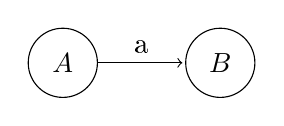
\begin{tikzpicture}[shorten >=1pt,node distance=2cm,on grid,auto] 
			\node[state] (A) {$A$}; 
			\node[state] (B) [right=of A] {$B$}; 
			\path[->] 
			(A) edge node {a} (B);
		\end{tikzpicture}
	\end{center}
	
	\item \framebox{$\prodrule{A}{\emptyword}$} , ahol $A \in N$.
	
	Az $\emptyword$ azt jelenti, hogy nem tud sehova sem tovább lépni. Ilyenkor \textbf{elfogadóállapot}ba érkezünk (vagy végállapotba). Vizualizálva:
	
	\begin{center}
		
\begin{tikzpicture}[shorten >=1pt,node distance=2cm,on grid,auto] 
			\node[state, accepting] (A) {$A$};
		\end{tikzpicture}
	\end{center}
\end{enumerate}

\newpage

\subsection{Véges nemdeterminisztikus automata determinisztikussá alakítása (VNDA $\to$ VDA)}

~\\[-2em]

\begin{mdframed}
	\textbf{Feladat}: Véges nemdeterminisztikus automatát (VNDA vagy NDA) alakítsuk át úgy, hogy determinisztikus legyen (VDA).
	
	\textbf{Előfeltétel}: Véges automata ($\mathcal{G}_3$-beli nyelvtanhoz).
\end{mdframed}

Adott az alábbi VNDA:
\begin{center}
	\setlength{\tabcolsep}{0.5em} % for the horizontal padding
	{\renewcommand{\arraystretch}{1.5}% for the vertical padding
	\begin{tabular}{cc||c|c}
		%\hline
		& $\delta$ & \texttt{a} & \texttt{b} \\
		\hline
		$\rightarrow$ & $S$ & $A$, $C$ &  \\
		%\hline
		$\leftarrow$ & $A$ & $A$ & $B$, $S$ \\
		%\hline
		& $B$ & $A$ & $C$, $S$ \\
		%\hline
		$\leftarrow$ & $C$ & $S$ &  \\
		%\hline
	\end{tabular}
	}
\end{center}

A $\rightarrow$ nyíl jelöli a kezdőállapotot, a $\leftarrow$ pedig az elfogadóállapotokat (más néven a végállapotokat). Nemdeterminisztikus automatával van dolgunk, ugyanis $S$-ből $A$-ba és $B$-be is eljuthatunk, melyek ugyanazt a terminálist eredményezik.

Írjuk fel halmazosan az \textbf{első sor}t. Az egyes halmazok fogják jelölni az állapotok ``címkéit'' (minta $q_1$ vagy $1$-ről lenne szó). Az új címkéket aláhúzással jelölöm. Minden egyes új címkét feldolgozunk.

\begin{center}
	\setlength{\tabcolsep}{0.5em} % for the horizontal padding
	{\renewcommand{\arraystretch}{1.5}% for the vertical padding
	\begin{tabular}{cc||c|c}
		%\hline
		& $\delta$ & \texttt{a} & \texttt{b} \\
		\hline
		$\rightarrow$ & $\{S\}$ & \dotuline{$\{A, C\}$} & \dotuline{$\emptyset$}
	\end{tabular}
	}
\end{center}

Dolgozzuk fel az új címkéket. Az eljárás hasonlít a BFS-re (szélességi gráfbejárásra).

Az $\{A,C\}$ halmaz elemei a táblázat szerint elfogadóállapotok, így a halmaz is megjelölhető ezzel a tulajdonsággal.

\begin{center}
	\setlength{\tabcolsep}{0.5em} % for the horizontal padding
	{\renewcommand{\arraystretch}{1.5}% for the vertical padding
		\begin{tabular}{cc||c|c}
			& $\delta$ & \texttt{a} & \texttt{b} \\
			\hline
			$\rightarrow$ & $\{S\}$ & \dotuline{$\{A, C\}$} & \dotuline{$\emptyset$} \\
			\hline
			$\leftarrow$ & $\{A, C\}$ & $\underbrace{\{A\}}_{A} \cup \underbrace{\{S\}}_C = \dotuline{\{A, S\}}$ & $\underbrace{\{B,S\}}_A \cup ~ \emptyset = \dotuline{\{ B,S \}}$ \\
			\hline
			& $ \emptyset$ & $\emptyset ~ \checkmark$ & $\emptyset ~ \checkmark$
		\end{tabular}
	}
\end{center}

Az $\{A,C\}$ halmaz két új halmazt, címkét eredményezett, így ezeket fel kell dolgoznunk.

Az üreshalmazból nyilvánvalóan egyik állapotba sem tudunk eljutni. Új halmaz sem jön létre, ezért feldolgozottnak jelöljük (kipipáljuk). Ha a hibát is jelezni akarjuk, akkor a(z) $\emptyset$-t kicserélhetjük egy $H$ hibahalmazra.

\begin{center}
	\setlength{\tabcolsep}{0.5em} % for the horizontal padding
	{\renewcommand{\arraystretch}{1.5}% for the vertical padding
		\begin{tabular}{cc||c|c}
			& $\delta$ & \texttt{a} & \texttt{b} \\
			\hline
			$\rightarrow$ & $\{S\}$ & \dotuline{$\{A, C\}$} & \dotuline{$\emptyset$ } \\
			\hline
			$\leftarrow$ & $\{A, C\}$ & $\dotuline{\{A, S\}}$ & $\dotuline{\{ B,S \}}$ \\
			\hline
			& $ \emptyset$ & $\emptyset ~ \checkmark$ & $\emptyset ~ \checkmark$ \\
			\hline
			$\leftarrow$ & $\{A,S\}$ & $\{A\} \cup \{C\} = \{A,C\} ~ \checkmark$ & $\emptyset \cup \{B,S\} = \{B,S\}$
		\end{tabular}
	}
\end{center}

Az $\{A,S\}$-ben van elfogadóállapot, így az egész megjelölhető annak. A halmaz nem hozott létre újabb halmazokat. Mivel az $\{A,C\}$-t korábban feldolgoztuk, ezért kipipálással megjelölöm. A $\{B,S\}$ meg amúgy is fel lett volna dolgozva a soron következő lépésben.

Hasonló lépésekkel végighaladunk az összes címkén. Ha elfogynak a halmazaink, az eljárás megáll.

\begin{center}
	\setlength{\tabcolsep}{0.5em} % for the horizontal padding
	{\renewcommand{\arraystretch}{1.5}% for the vertical padding
		\begin{tabular}{cc||c|c}
			& $\delta$ & \texttt{a} & \texttt{b} \\
			\hline
			$\rightarrow$ & $\{S\}$ & \dotuline{$\{A, C\}$} & \dotuline{$\emptyset$ } \\
			\hline
			$\leftarrow$ & $\{A, C\}$ & $\dotuline{\{A, S\}}$ & $\dotuline{\{ B,S \}}$ \\
			\hline
			& $ \emptyset$ & $\emptyset ~ \checkmark$ & $\emptyset ~ \checkmark$ \\
			\hline
			$\leftarrow$ & $\{A,S\}$ & $\{A\} \cup \{C\} = \{A,C\} ~ \checkmark$ & $\emptyset \cup \{B,S\} = \{B,S\}$ \\
			\hline
			& $\{B,S\}$ & $\{A\} \cup \{A,C\} = \{A,C\}$ & $\{C,S\} \cup \emptyset = \dotuline{\{C,S\}}$ \\
			\hline
			$\leftarrow$ & $\{C,S\}$ & $\{S\} \cup \{A,C\} = \dotuline{\{A,C,S\}}$ & $\emptyset \cup \emptyset = \emptyset$ \\
			\hline
			$\leftarrow$ & $\{A,C,S\}$ & $\{A\} \cup \{S\} \cup \{A,C\} = \{A,C,S\} ~ \checkmark$ & $\{B,S\} \cup \emptyset \cup \emptyset = \{B,S\}$
		\end{tabular}
	}
\end{center}

A kapott táblázatunk a bal oldalon található. Gyakran átnevezzük, átcímkézzük ezeket a halmazokat a könnyebb olvashatóság kedvéért számjegyekkel. Ez analóg a $q_0, q_1, \dots$ jelöléssel.

\begin{minipage}{0.5\linewidth}
	\begin{center}
		\setlength{\tabcolsep}{0.5em} % for the horizontal padding
		{\renewcommand{\arraystretch}{1.5}% for the vertical padding
			\begin{tabular}{cc||c|c}
				& $\delta$ & \texttt{a} & \texttt{b} \\
				\hline
				$\rightarrow$ & $\{S\}$ & $\{A, C\}$ & $\emptyset$ \\
				\hline
				$\leftarrow$ & $\{A, C\}$ & $\{A, S\}$ & $\{ B,S \}$ \\
				\hline
				& $ \emptyset$ & $\emptyset$ & $\emptyset$ \\
				\hline
				$\leftarrow$ & $\{A,S\}$ & $\{A,C\}$ & $\{B,S\}$ \\
				\hline
				& $\{B,S\}$ & $\{A,C\}$ & $\{C,S\}$ \\
				\hline
				$\leftarrow$ & $\{C,S\}$ & $\{A,C,S\}$ & $\emptyset$ \\
				\hline
				$\leftarrow$ & $\{A,C,S\}$ & $\{A,C,S\}$ & $\{B,S\}$
			\end{tabular}
		}
	\end{center}
\end{minipage}
\begin{minipage}{0.5\linewidth}
	\begin{center}
		\setlength{\tabcolsep}{0.5em} % for the horizontal padding
		{\renewcommand{\arraystretch}{1.5}% for the vertical padding
			\begin{tabular}{cc||c|c}
				& $\delta$ & \texttt{a} & \texttt{b} \\
				\hline
				$\rightarrow$ & 1 & 2 & 3 \\
				\hline
				$\leftarrow$ & 2 & 4 & 5 \\
				\hline
				& 3 & 3 & 3 \\
				\hline
				$\leftarrow$ & 4 & 2 & 5 \\
				\hline
				& 5 & 2 & 6 \\
				\hline
				$\leftarrow$ & 6 & 7 & 3 \\
				\hline
				$\leftarrow$ & 7 & 7 & 5
			\end{tabular}
		}
	\end{center}
\end{minipage}

\newpage

\subsection{Véges determinisztikus automata (VDA) minimalizálása}

~\\[-2em]

\begin{mdframed}
	\textit{Más néven}: minimális automata előállítása, VDA összefüggővé tétele.
	
	\textbf{Feladat}: VDA-ban az ekvivalens állapotokat egybeolvasztjuk -- azaz, azon állapotokat, melyek azonos szóra azonos eredményt adnak.
	
	\textbf{Előfeltétel}: VDA (feltételezzük, hogy megszabadultunk a nemdeterminisztikus jellegétől).
\end{mdframed}

Vegyük az alábbi VDA-t:\footnote{\textbf{Vigyázat}: Ez nem ugyanaz, mint amit az előző feladatban kaptunk.}

\begin{center}
	\setlength{\tabcolsep}{1em} % for the horizontal padding
	{\renewcommand{\arraystretch}{1.25}% for the vertical padding
		\begin{tabular}{cc||c|c}
			& $\delta$ & \texttt{a} & \texttt{b} \\
			\hline
			$\rightarrow$ & 1 & 4 & 5 \\
			%\hline
			$\leftarrow$ & 2 & 3 & 4 \\
			%\hline
			$\leftarrow$ & 3 & 2 & 8 \\
			%\hline
			& 4 & 9 & 2 \\
			%\hline
			& 5 & 2 & 3 \\
			%\hline
			& 6 & 8 & 7 \\
			%\hline
			& 7 & 8 & 1 \\
			& 8 & 9 & 3 \\
			$\leftarrow$ & 9 & 9 & 9
		\end{tabular}
	}
\end{center}

A $\delta$-relációra tekinthetünk úgy, mint egy olyan irányított gráfra, melynek mindegyik csúcsának fokszáma 2 és az élei fel vannak címkézve. 

Első lépésként meg kell határoznunk azon állapotokat (azaz a gráf azon csúcssait), amik elérhetők közvetett módon a kezdőállapotból (startcsúcsból). Ez a \textbf{BFS}-t vagy \textbf{szélességi gráfbejárás}t fogja jelenteni.\footnote{Fontos kiemelni, hogy a mi esetünkben nem egyszerű gráfról van szó, ugyanis hurokéleket tartalmaz. Emiatt szigorú értelemben arra számíthatunk, hogy az az algoritmus, amit \textit{Algoritmusok és adatszerkezetek II}.-n tanultunk, elakadhat emiatt. Ennek ellenére mégis ezt a szemléltetést fogom alkalmazni. Az az érvem mellette, hogy ha olyan csúcsot fedezünk fel, melynek van hurokéle, a $\pi$-címkéjének átállítása után másodjára nem fog bekerülni a $Q:Queue$ sorba, ezért mégsem fog komoly gondot jelenteni.}

\begin{center}
	\begin{tiny}
		\setlength{\tabcolsep}{0.5em} % for the horizontal padding
		{\renewcommand{\arraystretch}{1.5}% for the vertical padding
			\begin{tabular}{|c|c|c|c|c|c|c|c|c|c|c|c|c|c|c|c|c|c|c|c|}
				\hline
				\multicolumn{9}{|c|}{$d(u)$ címkék} & \multirow{3}{*}{$u:d(u)$} & \multirow{2}{*}{$Q : Queue$}  &  \multicolumn{9}{|c|}{$\pi(u)$ címkék}  \\
				\cline{1-9} \cline{12-20}
				1 & 2 & 3 & 4 & 5 & 6 & 7 & 8 & 9 & &  & 1 & 2 & 3 & 4 & 5 & 6 & 7 & 8 & 9 \\
				\cline{1-9} \cline{11-20}
				0 & $\infty$ & $\infty$ & $\infty$ & $\infty$ & $\infty$ & $\infty$ & $\infty$ & $\infty$ & & $\langle 1 \rangle$ & $\NIL$ & $\NIL$ & $\NIL$ & $\NIL$ & $\NIL$ & $\NIL$ & $\NIL$ & $\NIL$ & $\NIL$ \\
				\hline
				&  &  & 1 & 1 &  &  &  &  & $1:0$ & $\langle4,5\rangle$ &  &  &  & 1 & 1 &  &  &  &  \\
				\hline
				& 2 &  &  &  &  &  &  & 2 & $4:1$ & $\langle5,2,9\rangle$ &  & 4 &  &  &  &  &  &  & 4 \\
				\hline
				&  & 3 &  &  &  &  &  &  & $5:1$ & $\langle2,9,3\rangle$ &  &  & 5 &  &  &  &  &  &  \\
				\hline
				&  &  &  &  &  &  &  &  & $2:2$ & $\langle9,3\rangle$ &  &  &  &  &  &  &  &  &  \\
				\hline
				&  &  &  &  &  &  &  &  & $9:2$ & $\langle3\rangle$ &  &  &  &  &  &  &  &  &  \\
				\hline
				&  &  &  &  &  &  & 4 &  & $3:3$ & $\langle8\rangle$ &  &  &  &  &  &  &  & 3 &  \\
				\hline
				&  &  &  &  &  &  &  &  & $8:4$ & $\langle\rangle$ &  &  &  &  &  &  &  &  &  \\
				\hline
				0 & 2 & 3 & 1 & 1 & $\infty$ & $\infty$ & 4 & 2 & \multicolumn{2}{|c|}{eredmény} & $\NIL$ & 4 & 5 & 1 & 1 & $\NIL$ & $\NIL$ & 3 & 4 \\
				\hline
			\end{tabular}
		}
	\end{tiny}
\end{center}

Megállapíthatjuk belőle, hogy ahol $d(u) = \infty \land \pi(u) = \NIL$, azon csúcsok nem elérhetők az 1-es startcsúcsból (kezdőállapotból). Tehát, a 6-os és 7-es állapotoktól könnyedén megszabadulhatunk.

Az 1-esből \textit{elérhető állapotokat felosztjuk} két halmazra: \textbf{nem-elfogadóállapotok} (azaz $\{1,4,5,8\}$) és \textbf{elfogadóállapotok} (azaz $\{2,3,9\}$) halmazára. Az, hogy melyek elfogadóállapotok, azokat a táblázatból könnyedén leolvashatjuk (``$\leftarrow$'' nyíllal vannak megjelölve).

Ezeket a halmazokat szeretnénk \textbf{finomítani}, más szóval \textbf{partícionáljuk} őket. Ez azt jelenti, hogy egyre több halmaz jön létre és az egyes halmazok elemszáma egyre csökken. A partícionálás a \textit{szavak hossza szerint} történik. A partíciók jele: $\boxed{\sim^i}$ vagy $\boxed{\partition{i}}$ , ahol $i = \ell(u)$ ($u \in L(A)$).

\newpage

~\\[-2em]
\hrule

\begin{minipage}{0.1\linewidth}
	~
\end{minipage}
\begin{minipage}{0.45\linewidth}
	\centering \textbf{Nem-elfogadóállapotok}
\end{minipage}
\begin{minipage}{0.45\linewidth}
	\centering \textbf{Elfogadóállapotok}
\end{minipage}

%~\\[-2em]
\hrule

\begin{minipage}{0.1\linewidth}
	$\partition{0}$ :
\end{minipage}
\begin{minipage}{0.45\linewidth}
	\[\{ 1,4,5,8 \} =: A\]
\end{minipage}
\begin{minipage}{0.45\linewidth}
	\[\{2,3,9\} =: B\]
\end{minipage}

%~

\hrule
\begin{minipage}{0.1\linewidth}
	$\partition{1}$ :
\end{minipage}
\begin{minipage}{0.45\linewidth}
	\begin{center}
		Felbontandó partíciók: $A$.
		
		~
		
		\begin{tabular}{c|cc}
			%\hline
			$\delta$ & \texttt{a} & \texttt{b} \\
			\hline
			1 & $4\in A$ & $5\in A$ \\
			%\hline
			4 & $9\in B$ & $2\in B$ \\
			%\hline
			5 & $2\in B$ & $3 \in B$ \\
			%\hline
			8 & $9 \in B$ & $3\in B$ \\
			%\hline
		\end{tabular}
	
		~
		
		Avagy ugyanez tömörebben.
		
		~
		
		\begin{tabular}{c|cc}
			%\hline
			$\delta$ & \texttt{a} & \texttt{b} \\
			\hline
			\textbf{1} & $\textbf{A}$ & $\textbf{A}$ \\
			%\hline
			4 & $B$ & $B$ \\
			%\hline
			5 & $B$ & $B$ \\
			%\hline
			8 & $B$ & $B$ \\
			%\hline
		\end{tabular}
	
		~
		
		Új partíciók: $\{1\}$; $\{4,5,8\}$.
	\end{center}	
\end{minipage}
\begin{minipage}{0.45\linewidth}
	\begin{center}
		Felbontandó partíciók: $B$.
		
		~
		
		\begin{tabular}{c|cc}
			%\hline
			$\delta$ & \texttt{a} & \texttt{b} \\
			\hline
			2 & $3 \in B$ & $4 \in A$ \\
			3 & $2 \in B$ & $8 \in A$ \\
			9 & $9 \in B$ & $9 \in B$ 
		\end{tabular}
	
		~
	
		Avagy ugyanez tömörebben.
		
		~
		
		\begin{tabular}{c|cc}
			%\hline
			$\delta$ & \texttt{a} & \texttt{b} \\
			\hline
			2 & $B$ & $A$ \\
			3 & $B$ & $A$ \\
			\textbf{9} & $\textbf{B}$ & $\textbf{B}$ 
		\end{tabular}
	
		~
		
		Új partíciók: $\{2,3\}$; $\{9\}$.
	\end{center}
\end{minipage}

%~

\hrule
\begin{minipage}{0.1\linewidth}
	$\partition{2}$ :
\end{minipage}
\begin{minipage}{0.45\linewidth}
	\[ \{1\}=: C; ~ \{4,5,8\}=:D \]
	\begin{center}
		Felbontandó partíciók: $D$.
		
		~
		
		\begin{tabular}{c|cc}
			%\hline
			$\delta$ & \texttt{a} & \texttt{b} \\
			\hline
			4 & $F$ & $E$ \\
			%\hline
			\textbf{5} & $\textbf{E}$ & $\textbf{E}$ \\
			%\hline
			8 & $F$ & $E$ \\
			%\hline
		\end{tabular}
		
		~
		
		Új partíciók: $\{1\}$; $\{4,8\}$; $\{8\}$.
	\end{center}
\end{minipage}
\begin{minipage}{0.45\linewidth}
	\[ \{2,3\}=: E; ~ \{9\}=:F \]
	\begin{center}
		Felbontandó partíciók: $E$.
		
		~
		
		\begin{tabular}{c|cc}
			%\hline
			$\delta$ & \texttt{a} & \texttt{b} \\
			\hline
			2 & $E$ & $D$ \\
			3 & $E$ & $D$ \\
		\end{tabular}
		
		~
		
		Itt nem történik finomodás, \\ marad minden a régiben.
	\end{center}
\end{minipage}

%~

\hrule

\begin{minipage}{0.1\linewidth}
	$\partition{3}$ :
\end{minipage}
\begin{minipage}{0.45\linewidth}
	\[ \{1\}=: C; ~ \{4,8\}=:G; ~ \{5\} =:H \]
	\begin{center}
		Felbontandó partíciók: $G$.
		
		~
		
		\begin{tabular}{c|cc}
			%\hline
			$\delta$ & \texttt{a} & \texttt{b} \\
			\hline
			4 & $G$ & $E$ \\
			8 & $G$ & $E$ \\
			%\hline
		\end{tabular}
		
		~
		
		Nem történt finomodás
	\end{center}
\end{minipage}
\begin{minipage}{0.45\linewidth}
	%\[ \{2,3\}=: E; ~ \{9\}=:F \]
	\begin{center}
		--
	\end{center}
\end{minipage}

~\\[-1em]

\hrule

~\\[-1.5em]

\hrule

Mivel $\partition{3}$ -ban ($\ell(u)=3$ szavakban) nem történt finomodás a nem-elfogadóállapotok esetében az előző lépéshez képest (az elfogadóállapotok meg korábban véget értek), így leáll az algoritmus. Újracímkézzük azon állapotokat, partíciókat, melyek több elemből állnak. Így 
\[ \{2,3\} \to 23; ~~~~ \{4,8\} \to 48. \] 

A minimális automata / minimalizált VDA pedig:

\begin{center}
	\setlength{\tabcolsep}{1em} % for the horizontal padding
	{\renewcommand{\arraystretch}{1.25}% for the vertical padding
		\begin{tabular}{cc||c|c}
			& $\delta$ & \texttt{a} & \texttt{b} \\
			\hline
			$\rightarrow$ & 1 & 48 & 5 \\
			& 48 & 9 & 23 \\
			$\leftarrow$ & 23 & 23 & 48 \\
			& 5 & 23 & 23 \\
			$\leftarrow$ & 9 & 9 & 9
		\end{tabular}
	}
\end{center}

\section{Fordítóprogramok}

\subsection{title}

\end{document}